\documentclass{article}
\usepackage[margin=1in]{geometry}
\usepackage[linesnumbered,ruled,vlined]{algorithm2e}
\usepackage{amsfonts}
\usepackage{amsmath}
\usepackage{amssymb}
\usepackage{amsthm}
\usepackage{enumitem}
\usepackage{fancyhdr}
\usepackage{hyperref}
\usepackage{minted}
\usepackage{multicol}
\usepackage{pdfpages}
\usepackage{standalone}
\usepackage[many]{tcolorbox}
\usepackage{tikz-cd}
\usepackage{transparent}
\usepackage{xcolor}
% \tcbuselibrary{minted}

\author{Nathan Solomon}

\newcommand{\fig}[1]{
    \begin{center}
        \includegraphics[width=\textwidth]{#1}
    \end{center}
}

% Math commands
\renewcommand{\d}{\mathrm{d}}
\DeclareMathOperator{\id}{id}
\DeclareMathOperator{\im}{im}
\DeclareMathOperator{\proj}{proj}
\DeclareMathOperator{\Span}{span}
\DeclareMathOperator{\Tr}{Tr}
\DeclareMathOperator{\tr}{tr}
\DeclareMathOperator{\ad}{ad}
\DeclareMathOperator{\ord}{ord}
%%%%%%%%%%%%%%% \DeclareMathOperator{\sgn}{sgn}
\DeclareMathOperator{\Aut}{Aut}
\DeclareMathOperator{\Inn}{Inn}
\DeclareMathOperator{\Out}{Out}
\DeclareMathOperator{\stab}{stab}

\newcommand{\N}{\ensuremath{\mathbb{N}}}
\newcommand{\Z}{\ensuremath{\mathbb{Z}}}
\newcommand{\Q}{\ensuremath{\mathbb{Q}}}
\newcommand{\R}{\ensuremath{\mathbb{R}}}
\newcommand{\C}{\ensuremath{\mathbb{C}}}
\renewcommand{\H}{\ensuremath{\mathbb{H}}}
\newcommand{\F}{\ensuremath{\mathbb{F}}}

\newcommand{\E}{\ensuremath{\mathbb{E}}}
\renewcommand{\P}{\ensuremath{\mathbb{P}}}

\newcommand{\es}{\ensuremath{\varnothing}}
\newcommand{\inv}{\ensuremath{^{-1}}}
\newcommand{\eps}{\ensuremath{\varepsilon}}
\newcommand{\del}{\ensuremath{\partial}}
\renewcommand{\a}{\ensuremath{\alpha}}

\newcommand{\abs}[1]{\ensuremath{\left\lvert #1 \right\rvert}}
\newcommand{\norm}[1]{\ensuremath{\left\lVert #1\right\rVert}}
\newcommand{\mean}[1]{\ensuremath{\left\langle #1 \right\rangle}}
\newcommand{\floor}[1]{\ensuremath{\left\lfloor #1 \right\rfloor}}
\newcommand{\ceil}[1]{\ensuremath{\left\lceil #1 \right\rceil}}
\newcommand{\bra}[1]{\ensuremath{\left\langle #1 \right\rvert}}
\newcommand{\ket}[1]{\ensuremath{\left\lvert #1 \right\rangle}}
\newcommand{\braket}[2]{\ensuremath{\left.\left\langle #1\right\vert #2 \right\rangle}}

\newcommand{\catname}[1]{{\normalfont\textbf{#1}}}

\newcommand{\up}{\ensuremath{\uparrow}}
\newcommand{\down}{\ensuremath{\downarrow}}

% Custom environments
\newtheorem{thm}{Theorem}[section]

\definecolor{probBackgroundColor}{RGB}{250,240,240}
\definecolor{probAccentColor}{RGB}{140,40,0}
\newenvironment{prob}{
    \stepcounter{thm}
    \begin{tcolorbox}[
        boxrule=1pt,
        sharp corners,
        colback=probBackgroundColor,
        colframe=probAccentColor,
        borderline west={4pt}{0pt}{probAccentColor},
        breakable
    ]
    \color{probAccentColor}\textbf{Problem \thethm.} \color{black}
} {
    \end{tcolorbox}
}

\definecolor{exampleBackgroundColor}{RGB}{212,232,246}
\newenvironment{example}{
    \stepcounter{thm}
    \begin{tcolorbox}[
      boxrule=1pt,
      sharp corners,
      colback=exampleBackgroundColor,
      breakable
    ]
    \textbf{Example \thethm.}
} {
    \end{tcolorbox}
}

\definecolor{propBackgroundColor}{RGB}{255,245,220}
\definecolor{propAccentColor}{RGB}{150,100,0}
\newenvironment{prop}{
    \stepcounter{thm}
    \begin{tcolorbox}[
        boxrule=1pt,
        sharp corners,
        colback=propBackgroundColor,
        colframe=propAccentColor,
        breakable
    ]
    \color{propAccentColor}\textbf{Proposition \thethm. }\color{black}
} {
    \end{tcolorbox}
}

\definecolor{thmBackgroundColor}{RGB}{235,225,245}
\definecolor{thmAccentColor}{RGB}{50,0,100}
\renewenvironment{thm}{
    \stepcounter{thm}
    \begin{tcolorbox}[
        boxrule=1pt,
        sharp corners,
        colback=thmBackgroundColor,
        colframe=thmAccentColor,
        breakable
    ]
    \color{thmAccentColor}\textbf{Theorem \thethm. }\color{black}
} {
    \end{tcolorbox}
}

\definecolor{corBackgroundColor}{RGB}{240,250,250}
\definecolor{corAccentColor}{RGB}{50,100,100}
\newenvironment{cor}{
    \stepcounter{thm}
    \begin{tcolorbox}[
        enhanced,
        boxrule=0pt,
        frame hidden,
        sharp corners,
        colback=corBackgroundColor,
        borderline west={4pt}{0pt}{corAccentColor},
        breakable
    ]
    \color{corAccentColor}\textbf{Corollary \thethm. }\color{black}
} {
    \end{tcolorbox}
}

\definecolor{lemBackgroundColor}{RGB}{255,245,235}
\definecolor{lemAccentColor}{RGB}{250,125,0}
\newenvironment{lem}{
    \stepcounter{thm}
    \begin{tcolorbox}[
        enhanced,
        boxrule=0pt,
        frame hidden,
        sharp corners,
        colback=lemBackgroundColor,
        borderline west={4pt}{0pt}{lemAccentColor},
        breakable
    ]
    \color{lemAccentColor}\textbf{Lemma \thethm. }\color{black}
} {
    \end{tcolorbox}
}

\definecolor{proofBackgroundColor}{RGB}{255,255,255}
\definecolor{proofAccentColor}{RGB}{80,80,80}
\renewenvironment{proof}{
    \begin{tcolorbox}[
        enhanced,
        boxrule=1pt,
        sharp corners,
        colback=proofBackgroundColor,
        colframe=proofAccentColor,
        borderline west={4pt}{0pt}{proofAccentColor},
        breakable
    ]
    \color{proofAccentColor}\emph{\textbf{Proof. }}\color{black}
} {
    \qed \end{tcolorbox}
}

\definecolor{noteBackgroundColor}{RGB}{240,250,240}
\definecolor{noteAccentColor}{RGB}{30,130,30}
\newenvironment{note}{
    \begin{tcolorbox}[
        enhanced,
        boxrule=0pt,
        frame hidden,
        sharp corners,
        colback=noteBackgroundColor,
        borderline west={4pt}{0pt}{noteAccentColor},
        breakable
    ]
    \color{noteAccentColor}\textbf{Note. }\color{black}
} {
    \end{tcolorbox}
}


\fancyhf{}
\setlength{\headheight}{24pt}

\date{\today}
\title{Math 132 Homework \#2}

\begin{document}
\maketitle

\begin{prob}
    Chapter I, section 6, exercise 2, parts a \& d
\end{prob}
\begin{center}
    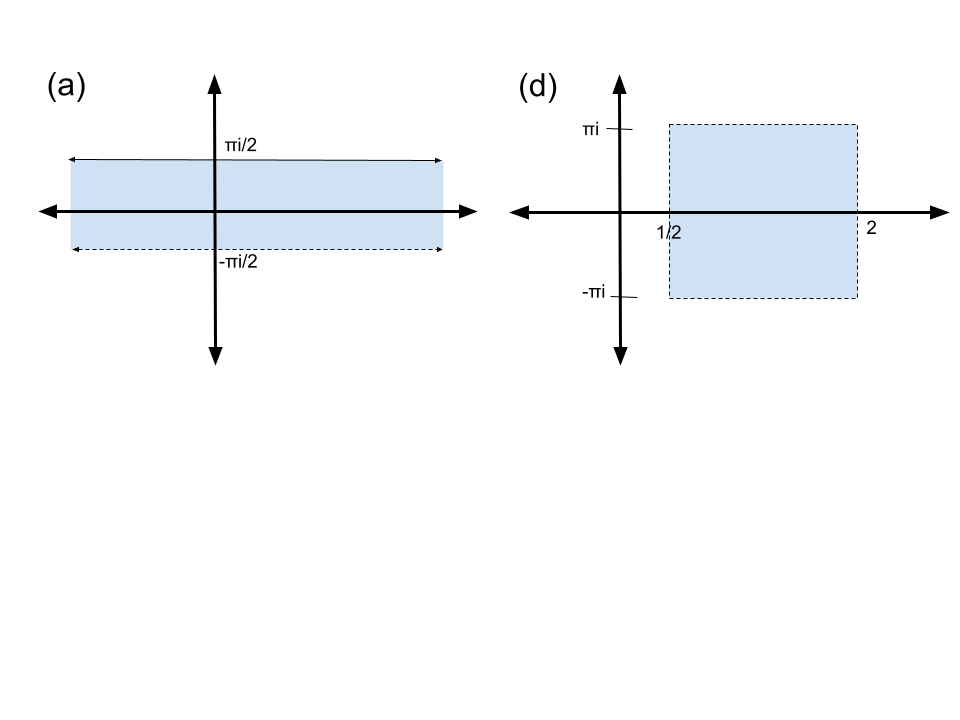
\includegraphics[width=\textwidth]{HW2 prob 1.png}
\end{center}


\bigskip
\par
\begin{prob}
    Chapter I, section 7, exercise 2
\end{prob}
\begin{align*}
    \log \left[ (1+i)^{2i} \right] &= \log \left[ \exp \left( 2i \log(1+i) \right) \right] \\
                                   &= \log \left[ \exp \left( 2i \cdot \left( \log(\sqrt{2}) + \frac{\pi i}{4} + 2\pi i k_1 \right) \right) \right] & k_1 \in \Z \\
                                   &= \left( 2i \cdot \left( \sqrt{2} + \frac{\pi i}{4} + 2\pi i k_1 \right) \right) +2\pi i k_2 & k_1, k_2 \in \Z \\
                                   &= i \log(2) - \frac{\pi}{2} - 4\pi k_1 + 2\pi i k_2 & k_1, k_2 \in \Z \\
                                   &= \left( - \frac{\pi}{2} 4\pi k_1 \right)  +i \left( \log(2)  + 2\pi k_2 \right)  & k_1, k_2 \in \Z.
\end{align*}
When you plot all possible values on the complex plane, you get one point (the ``principal value") at $z = -\pi/2 + 2 \log(2) i$, and infinitely many copies of that point in a grid with vertical spacing of $2 \pi$ and horizontal spacing of $4 \pi$.

\bigskip
\par
\begin{prob}
    Chapter I, section 8, exercise 1
\end{prob}
\begin{align*}
    \cos z \cos w - \sin z \sin w &= \left( \frac{e^{iz}+e^{-iz}}{2} \right) \left( \frac{e^{iw}+e^{-iw}}{2} \right) - \left( \frac{e^{iz}-e^{-iz}}{2i} \right) \left( \frac{e^{iw}-e^{-iw}}{2i} \right) \\
                                  &= \frac{1}{4} \left[ (e^{iz}+e^{-iz})(e^{iw}+e^{-iw})+(e^{iz}-e^{-iz})(e^{iw}-e^{-iw}) \right] \\
                                  &= \frac{1}{4} \left[ 2e^{iz}e^{iw} + 2e^{-iz}e^{-iw} \right] \\
                                  &= \cos (z+w). \\
    \sin z \cos w + \cos z \sin w &= \left( \frac{e^{iz}-e^{-iz}}{2i} \right) \left( \frac{e^{iw}+e^{-iw}}{2} \right) - \left( \frac{e^{iz}+e^{-iz}}{2} \right) \left( \frac{e^{iw}-e^{-iw}}{2i} \right) \\
                                  &= \frac{1}{4i} \left[ (e^{iz}-e^{-iz})(e^{iw}+e^{-iw})-(e^{iz}+e^{-iz})(e^{iw}-e^{-iw}) \right] \\
                                  &= \frac{1}{4i} \left[ 2e^{iz}e^{iw} - 2e^{-iz}e^{-iw} \right] \\
                                  &= \sin (z+w). \\
    \cosh (z+w) &= \cos(iz+iw) \\
                &= \cos(iz)\cos(iw)-\sin(iz)\sin(iw) \\
                &= (\cosh z) (\cosh w) - (i \sinh z)(i \sinh w) \\
                &= \cosh z \cosh w + \sinh z \sinh w. \\
    \sinh(z+w) &= -i \sin(iz+iw) \\
               &= -i \left( \sin(iz)\cos(iw) + \cos(iz)\sin(iw) \right) \\
               &= -i \left( (i \sinh z)(\cosh w) + (\cosh z)(i \sinh w) \right) \\
               &= \sinh z \cosh w + \cosh z \sinh w.
\end{align*}

\bigskip
\par
\begin{prob}
    Chapter I, section 8, exercise 2
\end{prob}
If $z=x+iy$, where $x,y \in \R$, then
\begin{align*}
    \abs{\cos z}^2 &= \abs{\cos(x+iy)}^2 \\
                   &= \abs{ \cos(x)\cos(iy)-\sin(x)\sin(iy) }^2 \\
                   &= \abs{ (\cos x)(\cosh y) - (\sin x)(i \sinh y) }^2 \\
                   &= \left( \cos x \cosh y \right)^2 + \left( \sin x \sinh y \right)^2 \\
                   &= \cos^2 x \cosh^2 y + \sin^2 x \sinh^2 y \\
                   &= \cos^2 x (\sinh^2 y + 1) + \sin^2 x \sinh^2 y \\
                   &= \cos^2 x + (\cos^2 x + \sin^2 x) \sinh^2 y \\
                   &= \cos^2 x + \sinh^2 y.
\end{align*}

\bigskip
\par
\begin{prob}
    Chapter II, section 1, exercise 2
\end{prob}
The sequence $z^n$ is bounded iff $ \abs{z}\leq 1$, because then all powers of $z$ also lie in the open unit disk.
\par
The sequence $z^n$ converges to zero iff $\abs{z}<1$, because then $\abs{z^n}=\abs{z}^n$, and we know the sequence $r^n$ converges to zero whenever $r \in (-1, 1)$.

\bigskip
\par
\begin{prob}
    Chapter II, section 1, exercise 15
\end{prob}
\begin{enumerate}[label=(\alph*)]
    \item Open
    \item Closed
    \item Open
    \item Neither open nor closed
    \item Open
    \item Neither open nor closed
    \item Open and closed
\end{enumerate}

\begin{center}
    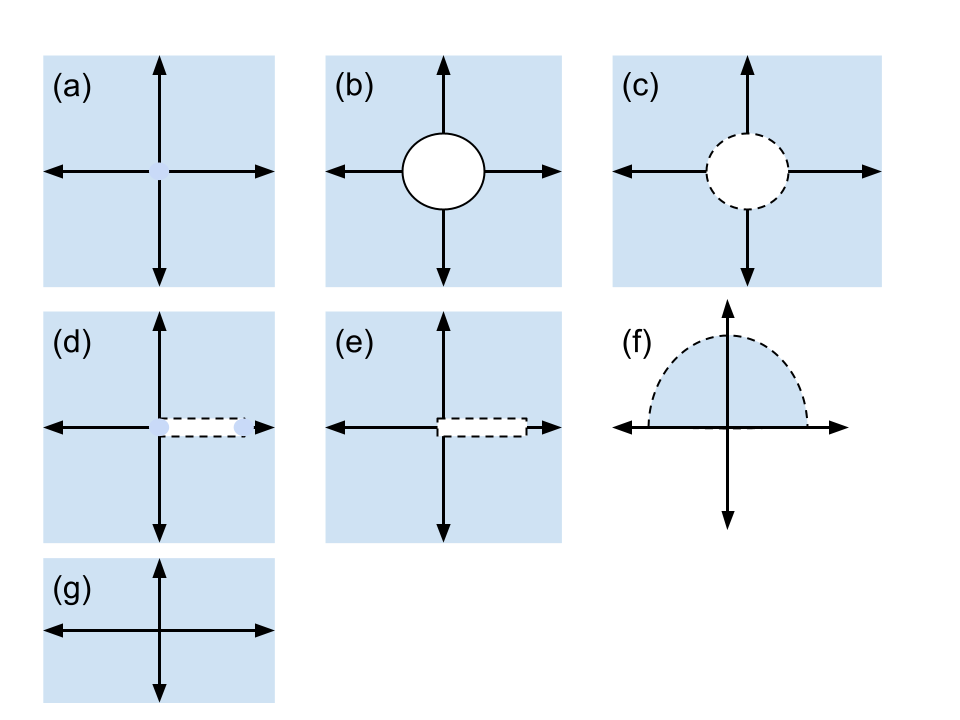
\includegraphics[width=\textwidth]{HW2 prob 6.png}
\end{center}


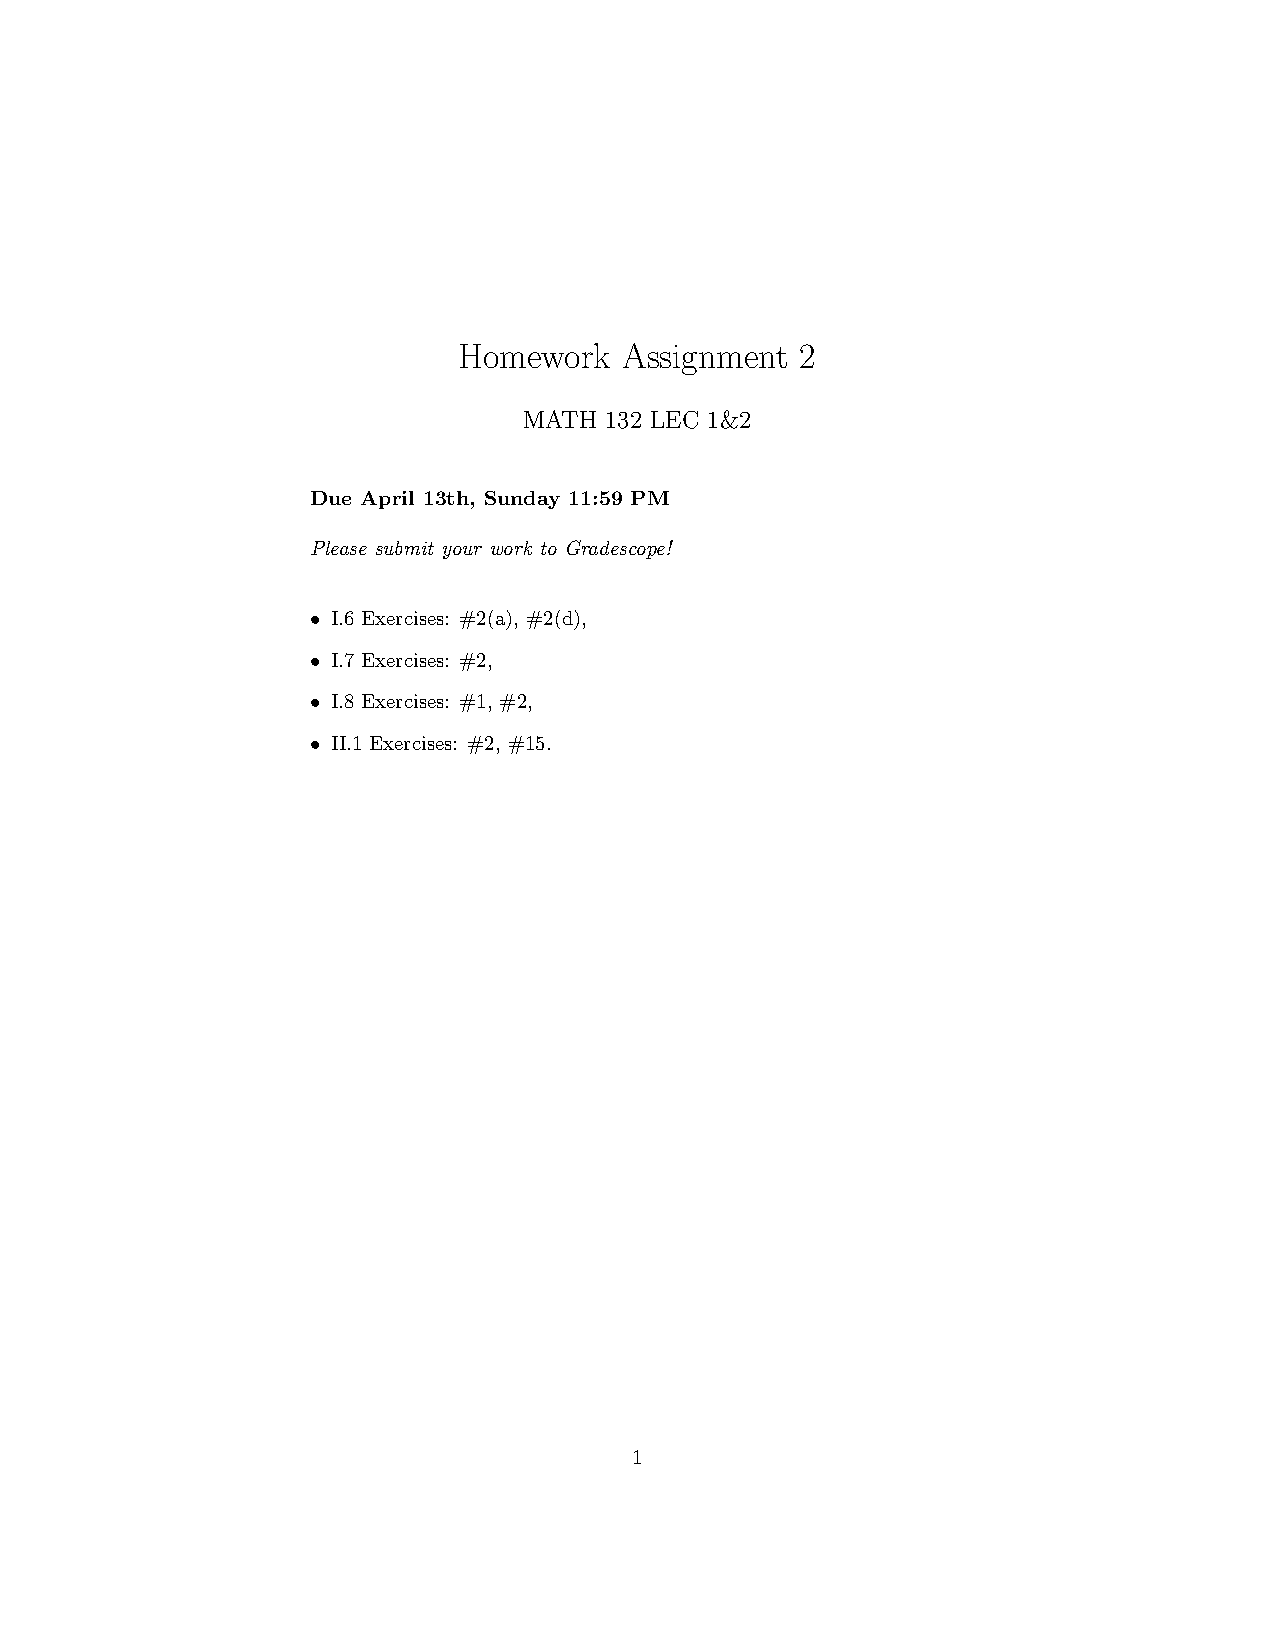
\includepdf[pages=-]{assignment.pdf}

\end{document}
